\documentclass[11pt, oneside]{article} 
\usepackage{geometry}
\geometry{letterpaper} 
\usepackage{graphicx}
	
\usepackage{amssymb}
\usepackage{amsmath}
\usepackage{parskip}
\usepackage{color}
\usepackage{hyperref}

\graphicspath{{/Users/telliott_admin/Tex/png/}}
% \begin{center} 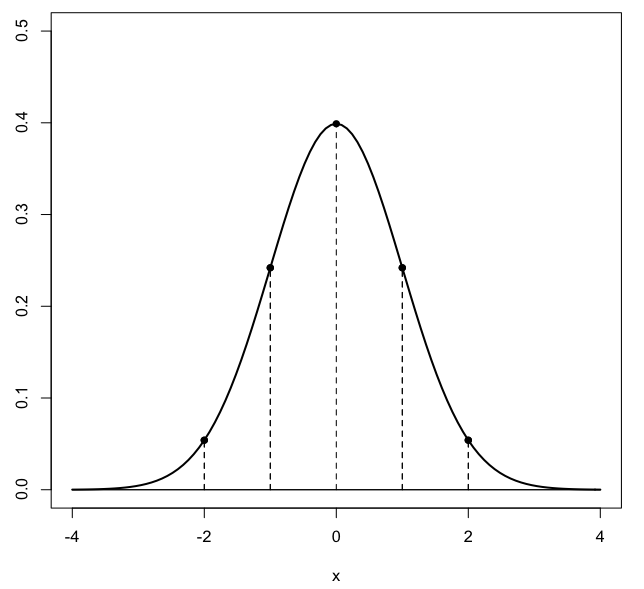
\includegraphics [scale=0.4] {gauss3.png} \end{center}

%break
\title{Related rates}
\date{}

\begin{document}
\maketitle
\Large

One simple form of related rates problem has two objects moving at right angles from each other, with positions and speeds given in terms of the origin. 

 For example:
"$A$ moves west at $x$ miles per hr, his current position is $x_0$ miles west of the origin, while $B$ moves south at $y$ miles per hr, and his current position is $y_0$ miles south of the origin.  At what rate are they moving apart?"

For the distance, we use Pythagoras:

\[ h^2 = x^2 + y^2 \]
All three values are functions of time so
\[ 2h h' = 2 x x' + 2 y y' \]
\[ h' = \frac{1}{h} (x x' + y y') \]
We will have to calculate $h$ from $x_0$ and $y_0$.

Another simple related rates problems involves two quantities with an equation relating the two quantities, e.g. the volume and radius of a sphere, where the sphere is a "balloon being inflated" or something

\[ V = \frac{4}{3} \pi r^3 \]
\[ \frac{dV}{dt} = 4 \pi r^2 \ \frac{dr}{dt} \]
or as usually stated in these problems
\[ V' = 4 \pi r^2 \ r' \]
If we know $V'$ and $r$ we can calculate $r'$.  Usually, rather than give you $r$ they will give you $V$, so then
\[ r = (\frac{4}{3} V)^{1/3} \]

A related problem :) is where the object is a cone (maybe inverted) and it's filling up with a fluid.  

\begin{center} 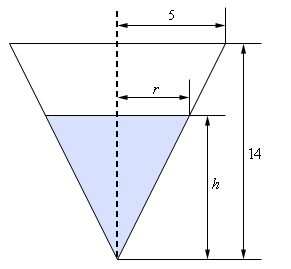
\includegraphics [scale=0.5] {cone_rates.png} \end{center}

Here, the formula for the volume of a cone is

\[ V = \frac{1}{3} \pi r^2 h \]

The problem is that since $r$ and $h$ depend on each other, we can't simply do 
\[ V' = \frac{1}{3} \pi r^2 h' \]
(this is wrong!)

In this case it's important to realize that the radius $r$ and the height $h$ of the fluid at its current level have the same ratio as the radius $R$ and height $H$ of the container.

\[ \frac{r}{h} = \frac{R}{H} \]
\[ r = \frac{R}{H} h \]
\[ h = \frac{H}{R} r \]

so we can substitute using the relationship between $r$ and $h$

\[ V = \frac{1}{3} \pi r^2 \frac{H}{R} r = \frac{1}{3} \pi \frac{H}{R} r^3 \]

Alternatively, we can eliminate $r$

\[ V = \frac{1}{3} \pi \frac{R^2}{H^2} h^3  \]

For example, with the figure above, ($R=5$ and $H=14$ feet), and given water is draining from the tank at $V'=-2 ft^3$ per hour

"At what rate is the depth of the water in the tank changing when the depth of the water is 6 ft?"

\[ V = \frac{1}{3} \pi \frac{R^2}{H^2} h^3  \]
\[ V' = \pi \frac{R^2}{H^2} h^2 h' \]

We're given $V'$ and $h$, $H$ and $R$, so can solve for $h'$.

The second question is "At what rate is the radius of the top of the water in the tank changing when the depth of the water is 6 ft?"

We need $r'$ given $h$ (and $R$, $H$, and $V'$)

\[ V = \frac{1}{3} \pi \frac{H}{R} r^3 \]
\[ V' = \pi \frac{H}{R} r^2 r' \]

\[ r = \frac{R}{H} h \]
\[ r^2 = (\frac{R}{H})^2 h^2 \]

Plugging in
\[ V' = \pi \frac{R}{H} h^2 r' \]
\vspace{10mm}

Here is another related rates problem.  An airplane and a parachutist are at the same height currently, and in the same direction as you look at them.  

\begin{center} 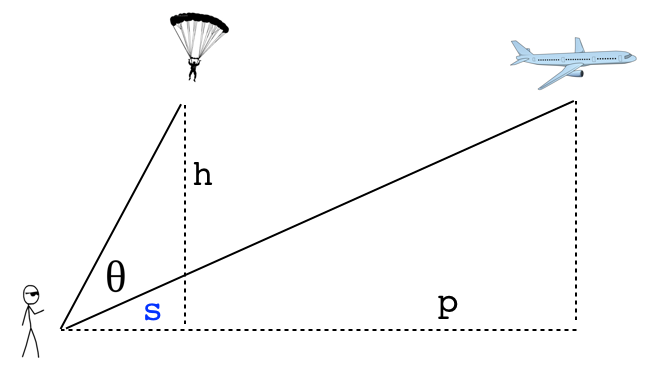
\includegraphics [scale=0.5] {rr1.png} \end{center}

The airplane moves away from you at $500$ ft/s.  The parachutist is floating downward at $-10$ ft/s and will land $1000$ ft away from you.  The current value of $h = 2000$ ft.  The current value of $p = 8000$ ft.  Find $d \theta/dt$.

\[ p(t) = p_0 + 500 t \]
\[ h(t) = h_0 - 10 t  \]
\[ p' = 500 \]
\[ h' = -10 \]

Find equations for the angles involved
\[ \tan s = \frac{2000}{p} \]
we use the constant value of $2000$ rather than $h$, which will vary.
\[ u = s + \theta \]
\[ \tan u = \frac{h}{1000} \]
Take the derivatives.  For the airplane
\[ \tan s = \frac{2000}{p} \]
\[ \frac{d}{dt} \tan s = \sec^2 s \frac{ds}{dt} = \frac{d}{dt} \frac{2000}{p}  = -2000 \frac{1}{p^2} \frac{dp}{dt}  \]
\[ \frac{ds}{dt} = -2000 \frac{1}{p^2} \frac{dp}{dt} \cos^2 s \]

In the above equation, we know $p=8000$ and $dp/dt = 500$.  We have to find the cosine.  If $\tan s=1/4$ then $\cos s = \sqrt{16/17}$.  
\[ \frac{ds}{dt} = -2000 \ \frac{1}{8000^2} \ 500 \ \frac{16}{17} \]
\[ \frac{ds}{dt} = -\frac{1}{4} \frac{1}{16} \frac{16}{17} = -\frac{1}{68} = - 0.0147\]

For the parachutist

\[ \frac{d}{dt} \tan u = \sec^2 u \frac{du}{dt} = \frac{d}{dt} \frac{h}{1000}  = \frac{1}{1000} \frac{dh}{dt}  \]
\[ \frac{du}{dt} = \frac{1}{1000} \frac{dh}{dt}  cos^2 u \]

In the above equation, we know $dh/dt = -10$.  We have to find the cosine.  If $\tan u=2$ then $\cos u = 1/\sqrt{5}$.  So
\[ \frac{du}{dt} = 0.001 \  (-10) \ \frac{1}{5}  = - 0.002 \]

Since $\theta = u - s$
\[ \frac{d \theta}{dt} = \frac{du}{dt} -  \frac{ds}{dt} = - 0.002 + 0.0147 =  0.0127 \]
The angle $\theta$ between plane and parachutist is \emph{increasing} with time (about 3/4 of a degree per second).

\end{document}  